\section{Introduction}

\begin{flushright}
{\em If you cannot---in the long run---tell everyone\\ what you have
been doing, your doing has been worthless.}\\ --- Schr\"odinger,
closing a 1950 public lecture~\cite{schrodinger51}
\end{flushright}

Scientists must write papers.\footnote{This paper obeys ASD-STE100
Simplified Technical English~\cite{asdste25}.
Where STE and the usual style rules of this project disagree, STE
wins.
For example, STE lets a sentence start with ``But.''}
Society gives science money, freedom, and trust.
In return, scientists must tell everyone what they found.
Institutions also count papers when they make decisions about money,
jobs, promotion, and graduation.
Thus, for one reason or the other, the writing must occur.

But writing is hard:
\begin{enumerate}
\item New writers need help with the craft of papers.
The known advice is scattered across many years of folklore.
Also, almost none of that advice has tool support.
\item When new writers ask large language models (LLMs) for help, the
models make text that is weak and long.
Many readers call this text ``AI slop.''\footnote{``Slop'' is
machine-made content of low quality, made in large
quantities~\cite{mw25slop}.
One study of 14 million PubMed abstracts found that an LLM touched at
least 10\% of the 2024 abstracts~\cite{kobak24}.
Software developers report the same problem with machine-made code and
documents~\cite{baltes26}.
The term has no agreed definition, but studies now map its
dimensions~\cite{shaib25}.}
\item Older researchers cannot find time for research, because paper
work fills their days.
In software engineering (SE), this load is large.
One SE paper costs more than four times the effort of one machine
learning paper (4.09 against 0.86 ICLR
points~\cite{luo25,menzies26se}).
\end{enumerate}

\begin{figure*}[t]
\centering
\begin{tabular}{c@{\hspace{0.5em}}c@{\hspace{0.8em}}c}
 & {\small\bf AI assistant} & {\small\bf shared document}\\[0.3em]
\raisebox{0.95in}{\small\bf\shortstack{browser only\\(rungs 1--2)}} &
\begin{tikzpicture}[inner sep=0]\node[anchor=south west] (i)
{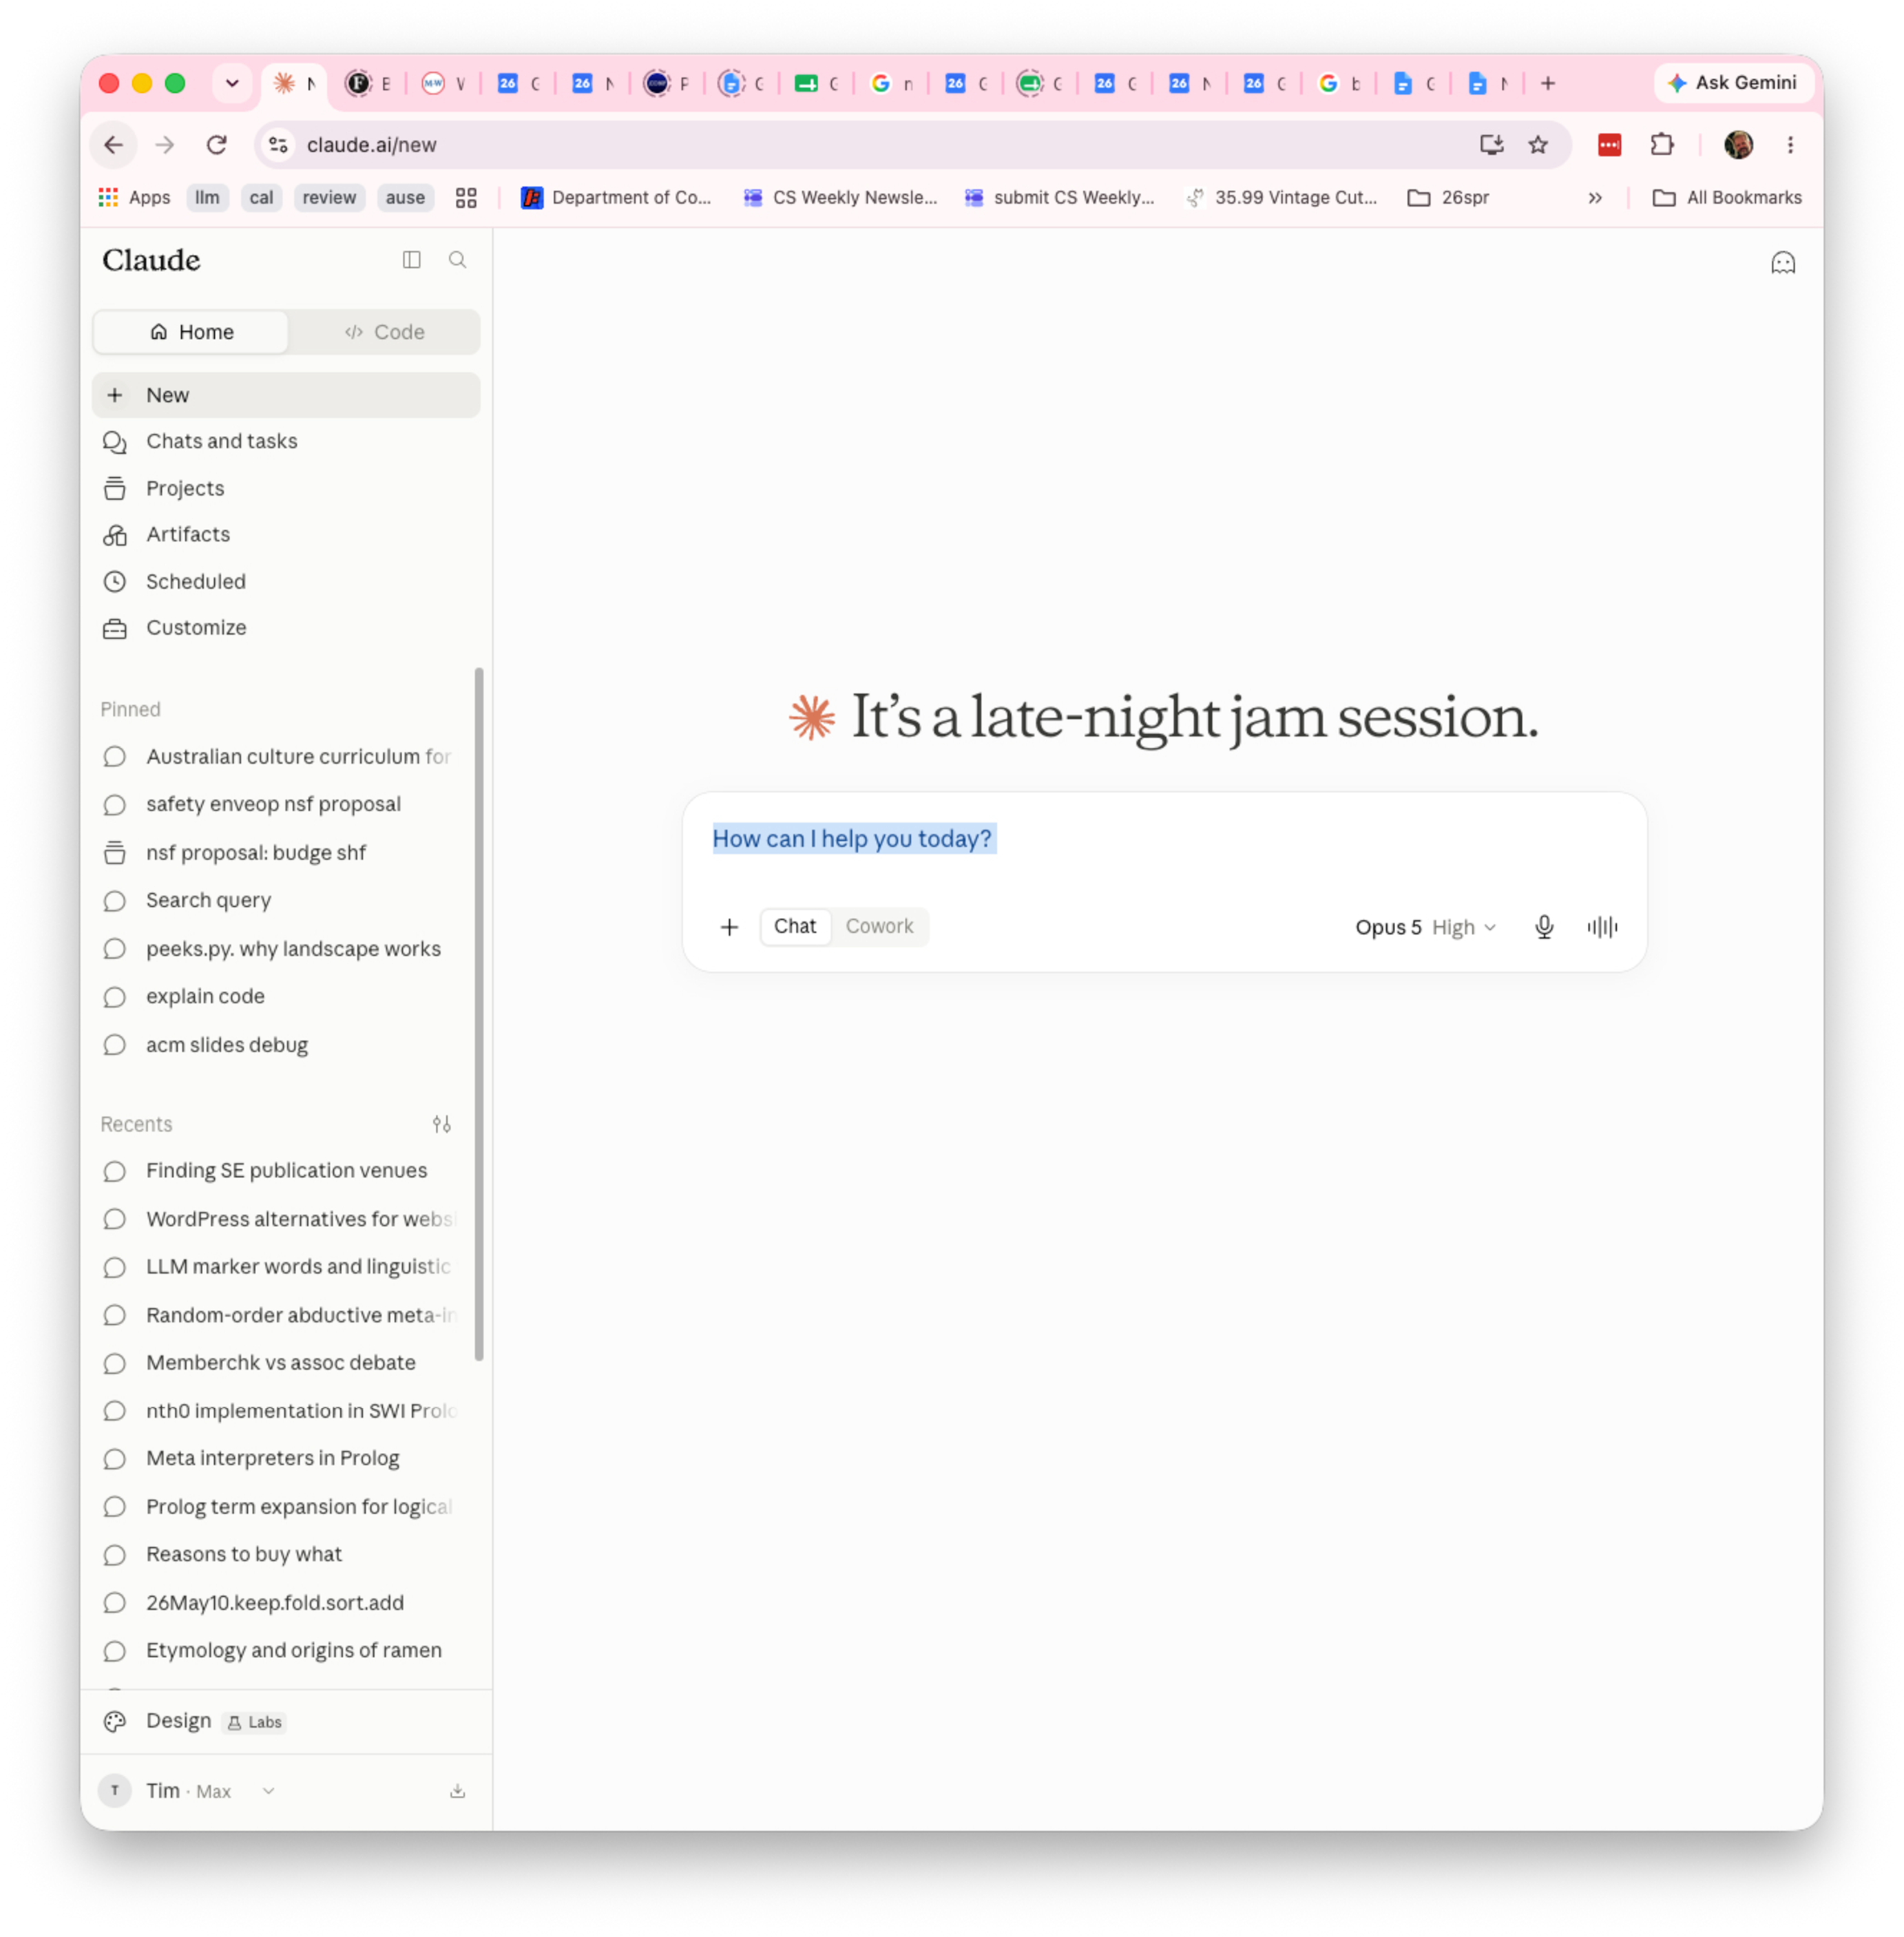
\includegraphics[height=1.9in]{fig/gemini}};\node[anchor=south
west, font=\fontsize{50}{50}\selectfont\bfseries, black] at
([xshift=4mm,yshift=4mm]i.south west) {A};\end{tikzpicture} &
\begin{tikzpicture}[inner sep=0]\node[anchor=south west] (i)
{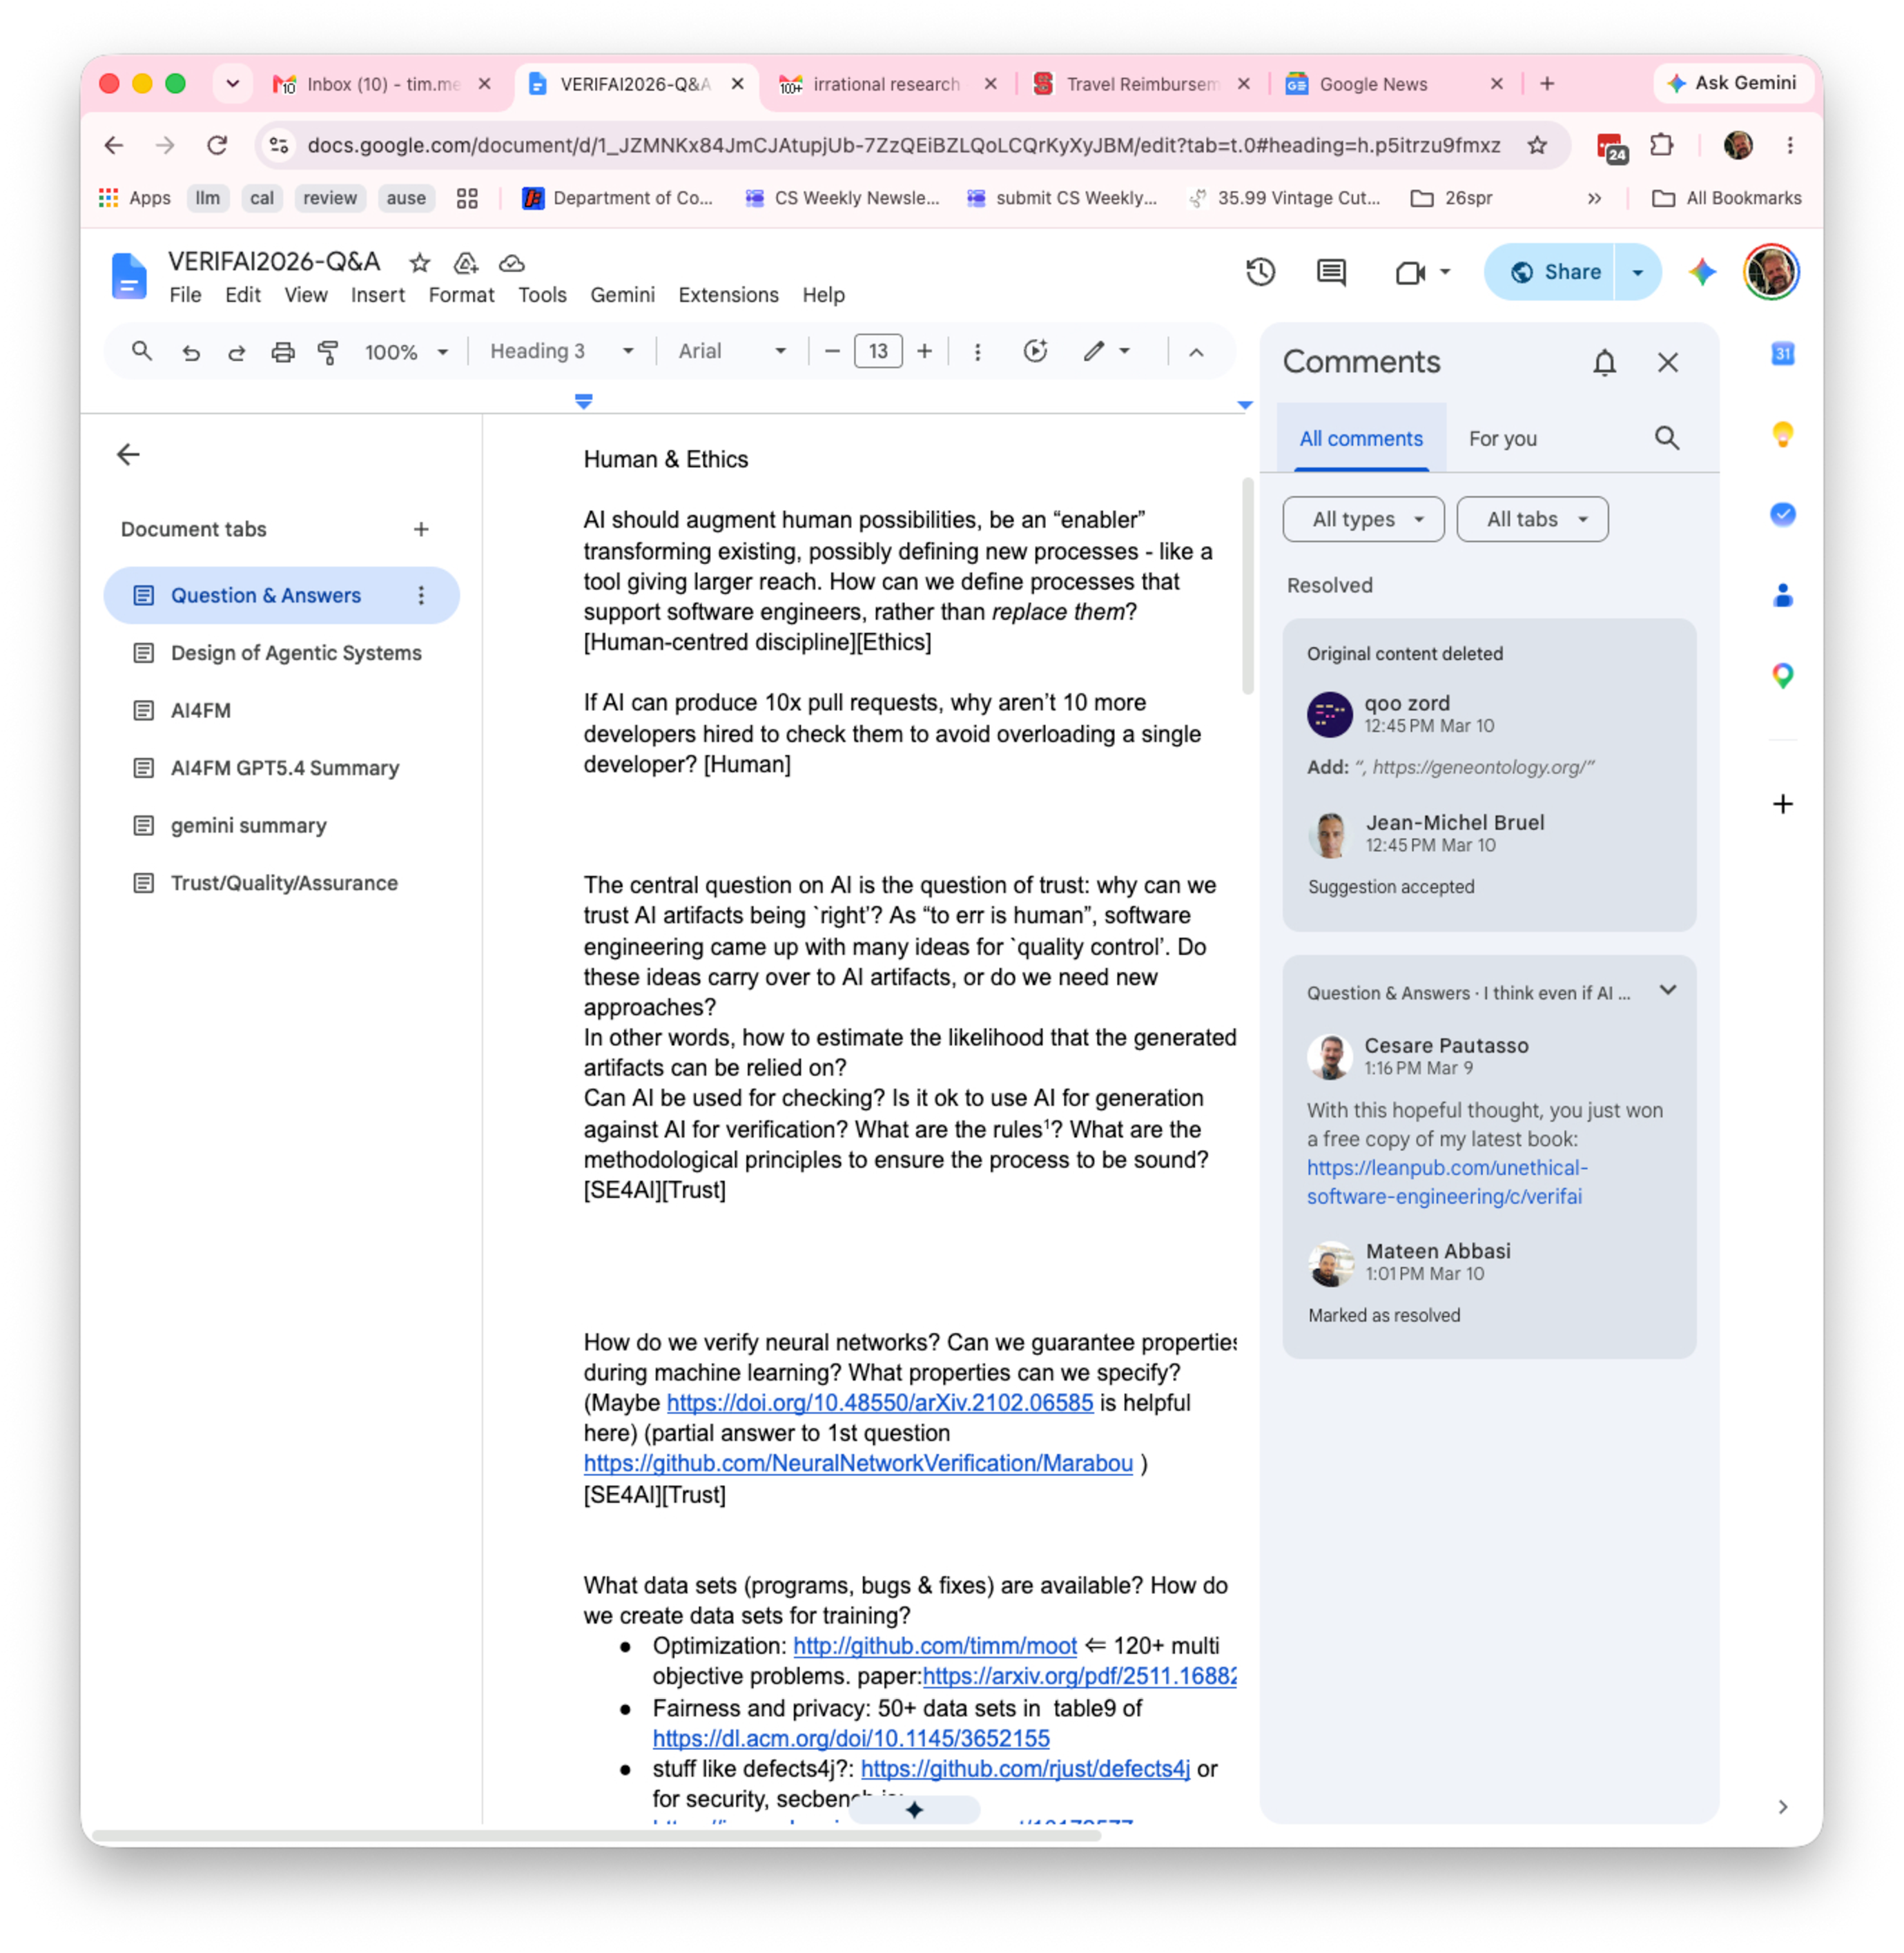
\includegraphics[height=1.9in]{fig/docs}};\node[anchor=south west,
font=\fontsize{50}{50}\selectfont\bfseries, black] at
([xshift=4mm,yshift=4mm]i.south west) {B};\end{tikzpicture}\\[0.6em]
\raisebox{0.95in}{\small\bf\shortstack{repository\\(rungs 3--4)}} &
\begin{tikzpicture}[inner sep=0]\node[anchor=south west] (i)
{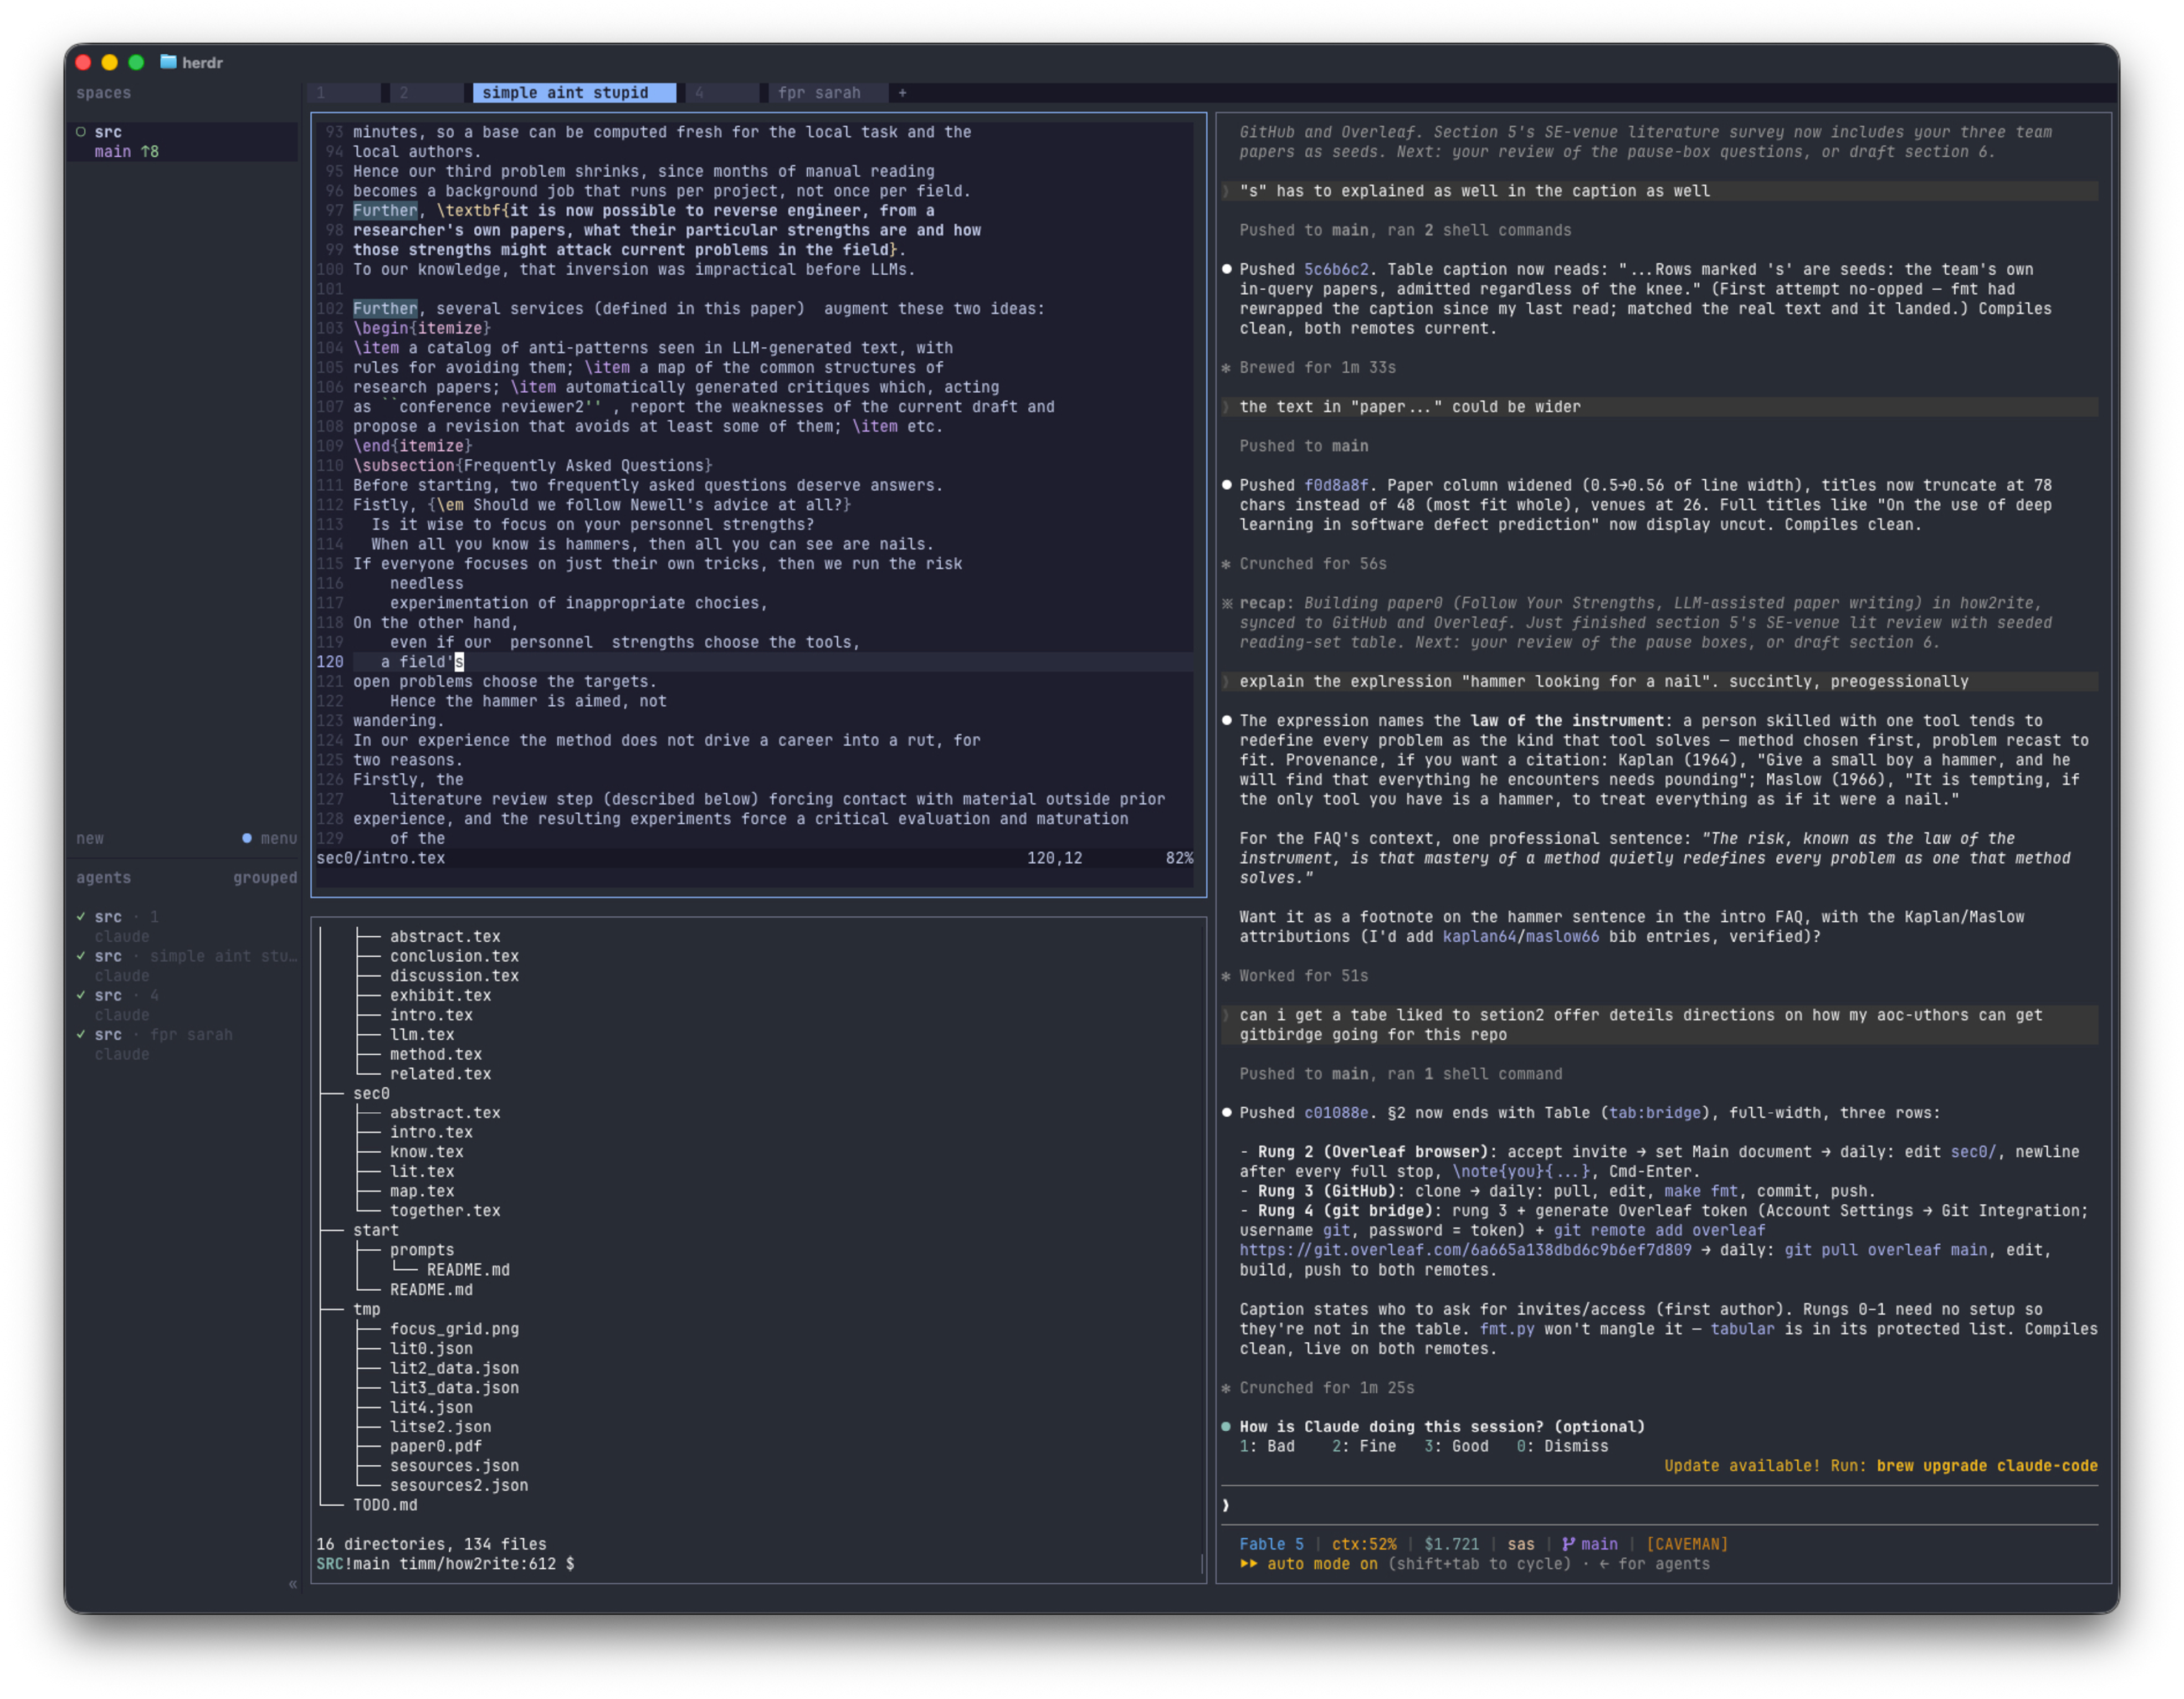
\includegraphics[height=1.9in]{fig/claude}};\node[anchor=south
west, font=\fontsize{50}{50}\selectfont\bfseries, white] at
([xshift=4mm,yshift=4mm]i.south west) {C};\end{tikzpicture} &
\begin{tikzpicture}[inner sep=0]\node[anchor=south west] (i)
{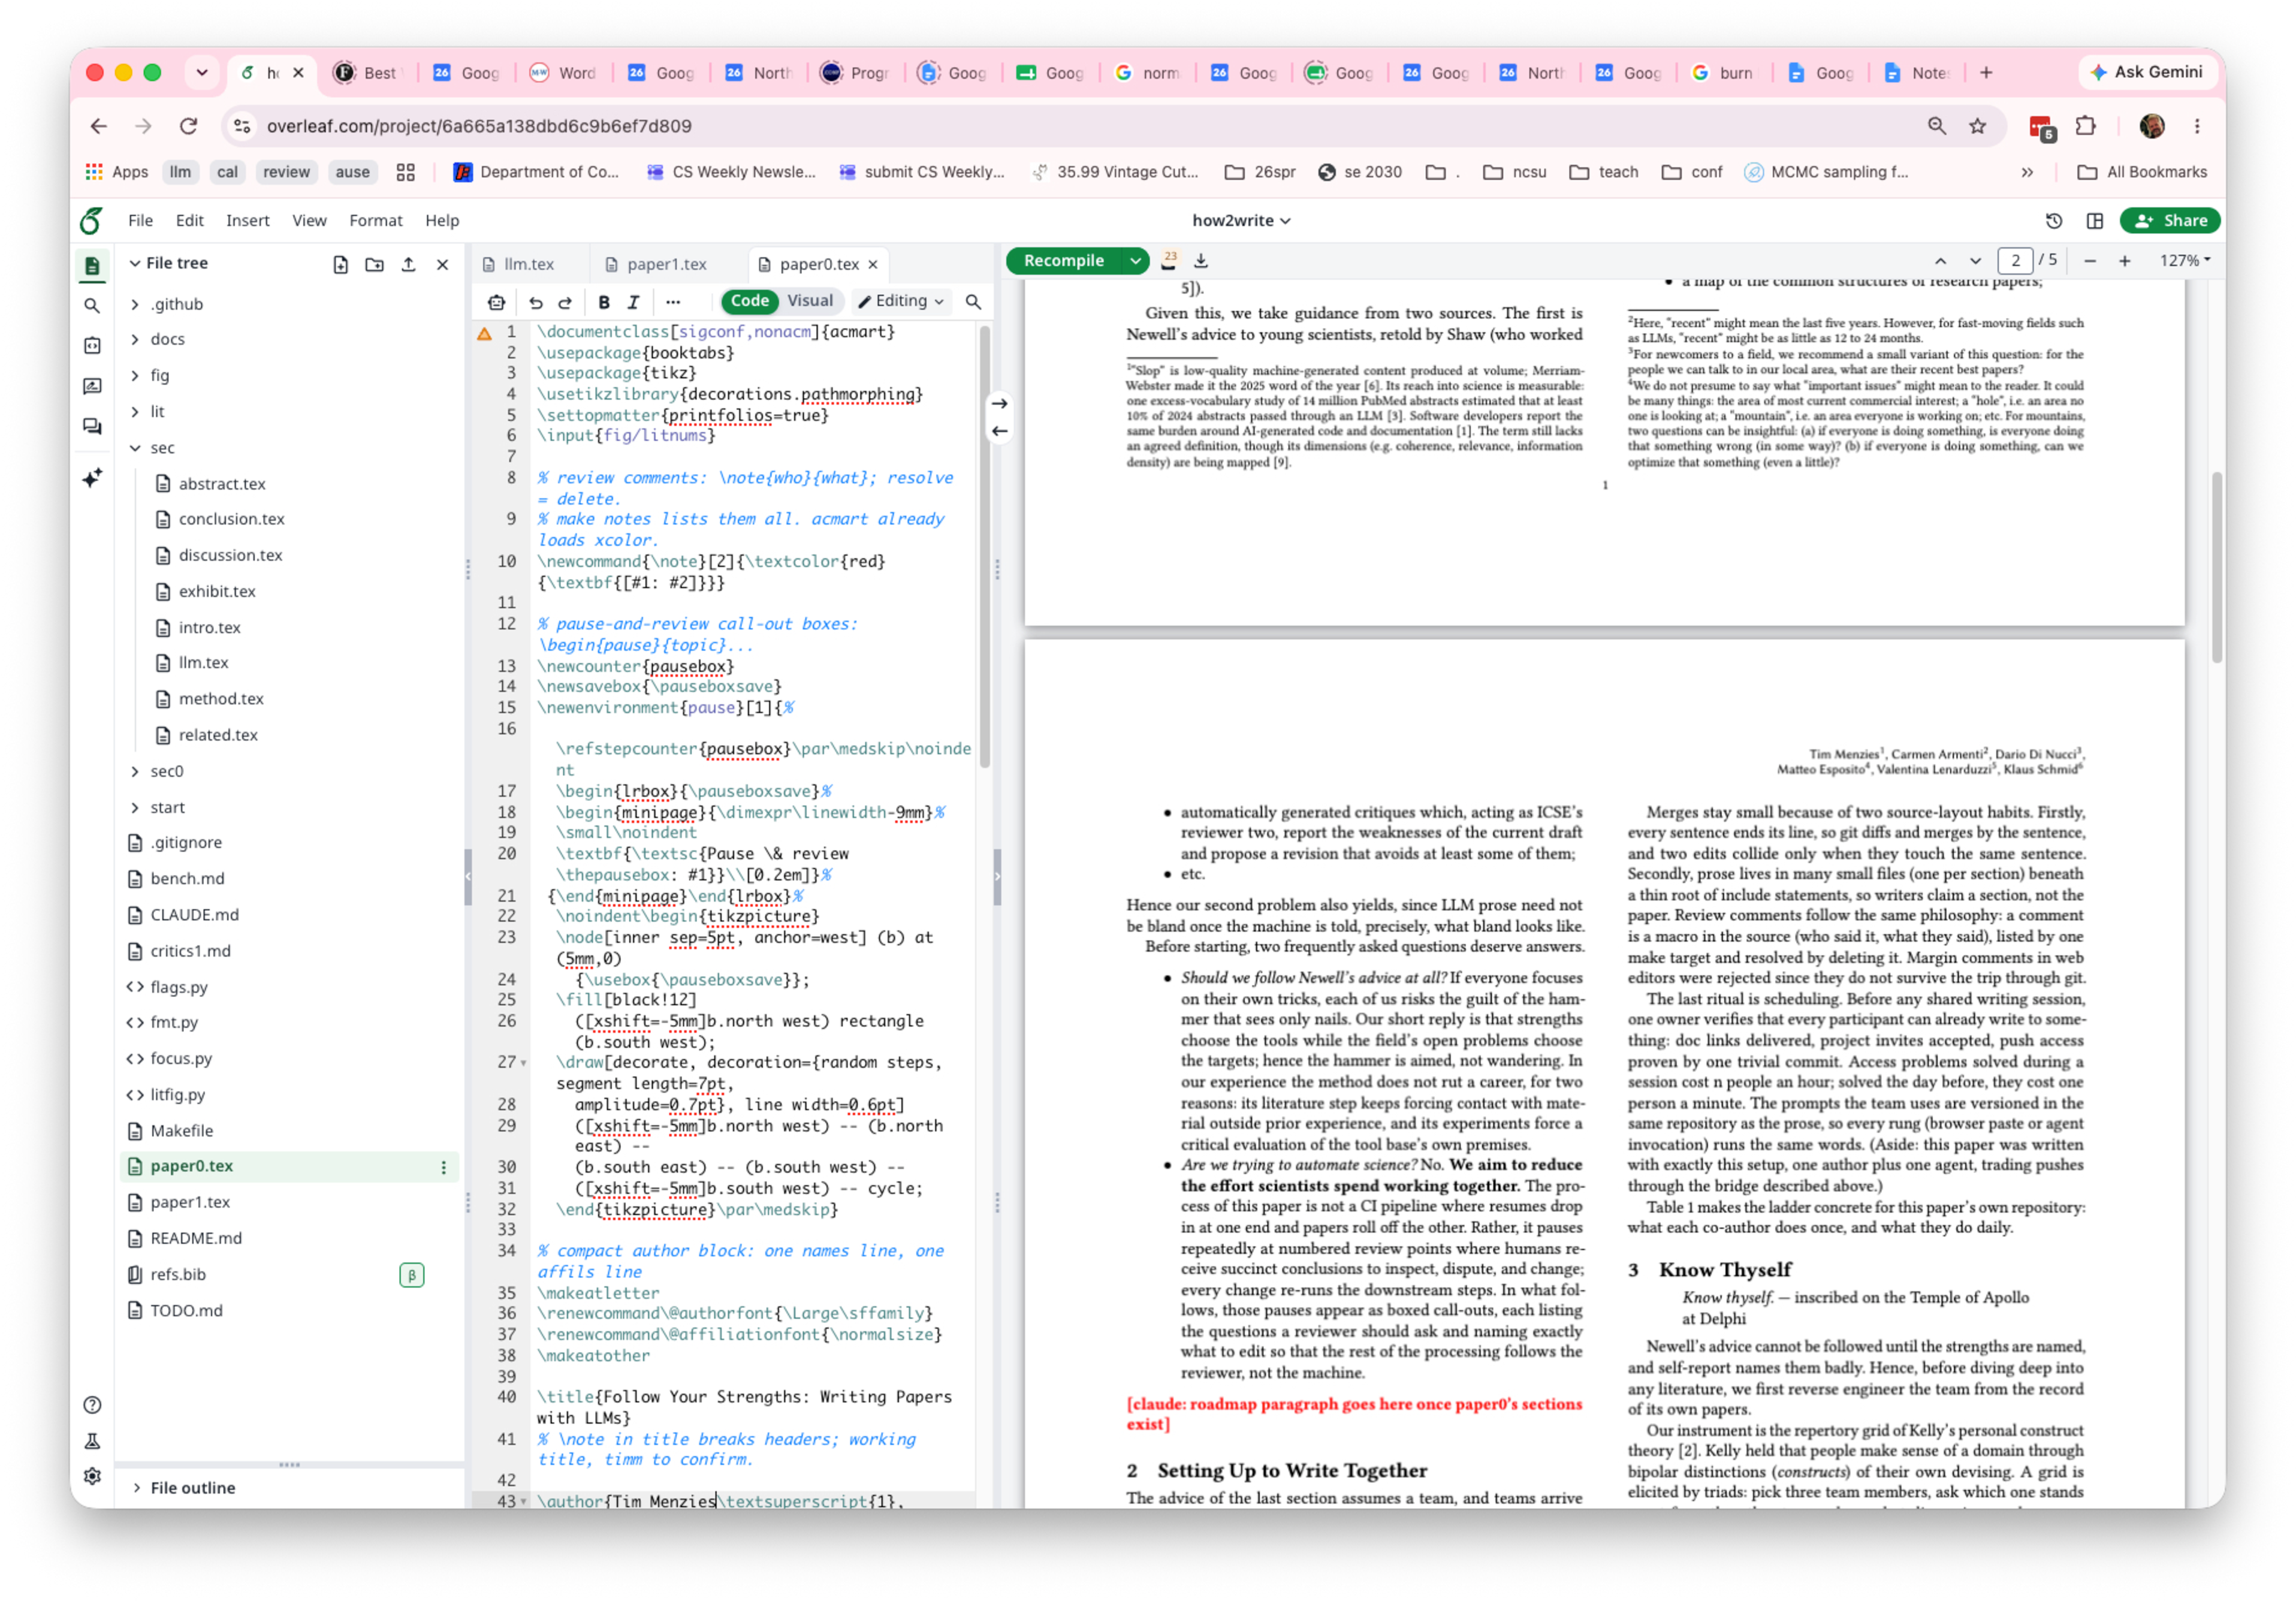
\includegraphics[height=1.9in]{fig/overleaf}};\node[anchor=south
west, font=\fontsize{50}{50}\selectfont\bfseries, black] at
([xshift=4mm,yshift=4mm]i.south west) {D};\end{tikzpicture}\\
\end{tabular}
\caption{Teams can use this advice in many ways.
The columns show AI assistants and shared documents.
The top row shows the browser tools of rungs 1 and 2 (A: Gemini, B:
Google Docs).
The bottom row shows the repository tools of rungs 3 and 4 (C: Claude
Code on the git bridge, D: Overleaf with the same paper).}
\label{fig:faces}
\end{figure*}

Given these problems, we take guidance from two sources.
The first source is the advice of Newell to young scientists.
Shaw worked with Newell at CMU.
She gave this advice again when she answered a question at her FSE'26
keynote~\cite{shaw26}:
\begin{quote}
{\em Know what you are good at.
Work from those strengths, not from your weaknesses.
Then point those strengths at whatever your field currently ranks as
its hardest open problems.} --- after Newell~\cite{newell91}
\end{quote}
Applied to paper writing, this advice gives a workflow of small steps.
It also gives teams a natural division of labor.
Four questions find that division:
\begin{enumerate}
\item ``Hello team: what are our recent best papers?''\footnote{Here,
``recent'' can mean the last five years.
But for fast fields, for example LLMs, ``recent'' can be 12 to 24
months.}
\item ``What do those papers show, through reverse engineering, as our
best strengths?''
\item ``Given those strengths, in which research areas can we work?''
\item ``How can our strengths attack the important issues of those
areas?''\footnote{We do not say what ``important issues'' means for
the reader.
It can be the area with the most commercial interest.
It can be a ``hole,'' an area where no one works.
It can be a ``mountain,'' an area where everyone works.
For mountains, two questions help: (a)~if everyone does one thing, do
they all do it incorrectly in some way?
(b)~if everyone does one thing, can we make that thing better, even a
little?}
\end{enumerate}
Thus, the four questions attack our first problem.
A workflow of clear steps is teachable.
Folklore is not.

The second source is an experience base.
An experience base is a database that machines make from the research
corpus.
It holds, for example:
\begin{itemize}
\item results at the state of the art; \item holes in that state of
the art; \item the test standards of each sub-field; \item other data
of this type.
\end{itemize}
This base is not one size for all.
With LLMs, machines can download and parse hundreds of papers in
minutes.
Thus, a team can compute a fresh base for each task and for each set
of authors.
This attacks our third problem, because months of reading become a
background job for each project.
Also, \textbf{machines can now find, from the papers of one
researcher, the strengths of that researcher}.
Before LLMs, this was not practical.

Several services help these two ideas:
\begin{itemize}
\item a catalog of anti-patterns in LLM text, with rules to avoid
them; \item a map of the usual structures of research papers; \item
automatic critiques that act as ``reviewer 2,'' report the weak points
of a draft, and propose a better draft; \item other services of this
type.
\end{itemize}
Thus, our second problem also becomes smaller.
LLM text does not need to be bland, if we tell the machine what bland
is.

Before we start, we answer two frequent questions.
\begin{itemize}
\item {\em Should we follow the advice of Newell?}
A person who only has a hammer sees only nails, and that is a risk.
But our strengths only select the tools.
The open problems of the field select the targets.
Also, the literature step pushes us to material outside our
experience.
The experiments test the premises of our own tools.
Thus, this method does not lock a career in one place.
\item {\em Do we try to automate science?}
No. \textbf{We try to decrease the effort that scientists spend when
they work together.}
This process is not a pipeline that eats resumes and makes papers.
The process stops at numbered review points.
At each point, a human reads a short conclusion, disputes it, or
changes it.
Each change runs the steps after it again.
\begin{pause}{Pause and reflect}
Boxed call-outs show these pauses.
Each box lists the questions for the reviewer.
Each box names the files to edit, so that the next steps follow the
reviewer, not the machine.
\end{pause}
\end{itemize}
